\documentclass{report}                                                           
        
\usepackage{titlesec}
\titleformat{\chapter}
  {\normalfont\LARGE\bfseries}{\thechapter}{1em}{}
\titlespacing*{\chapter}{0pt}{3.5ex plus 1ex minus .2ex}{2.3ex plus .2ex}
\usepackage[left=1in, right=1in, top=1in, bottom=1in]{geometry}
\usepackage{hyperref} 
\usepackage{xcolor} 
\usepackage{ulem}                     
\usepackage{graphicx} 
\usepackage{rotating}
\usepackage{setspace}
\usepackage{longtable}
\usepackage[acronym]{glossaries}
\usepackage[binary-units=true]{siunitx}
\usepackage{multirow}
\usepackage{subcaption}
                                                                                 
\newcommand{\note}[1]{\textcolor{blue}{\textit{note}: #1}}                       
\newcommand{\tristan}[1]{\textcolor{red}{TG: #1}}                                
\newcommand{\weird}[1]{\uwave{#1}}  

\newacronym{hpc}{HPC}{High Performance Computing}
\newacronym{fuse}{FUSE}{Filesystem in User Space}
\newacronym{hdfs}{HDFS}{Hadoop Distributed File System}
\newacronym{ost}{OST}{object storage target}
\newglossaryentry{ml}{
    name = $M\_{l}$ ,
  description = The makespan with page cache,
}


% Fix link colors
\hypersetup{
    colorlinks = true,
    linkcolor=red,
    citecolor=red,
    urlcolor=blue,
    linktocpage % so that page numbers are clickable in toc
}
\setcounter{tocdepth}{1}

\makenoidxglossaries
\begin{document} 
    \begin{titlepage}
       \begin{center}

           \hspace{0pt}
                \vfill
                    \textbf{Porting Big Data optimizations to scientific workflows on HPC}
                \vfill
           \hspace{0pt}

           \vspace{2cm}

           \textbf{Valerie Hayot-Sasson}

           \vfill

           ENCS 8011: Graduate Seminar\\

           \vspace{0.8cm}

           Department of Software Engineering and Computer Science\\
           Concordia University\\
           \today

       \end{center}
    \end{titlepage}
    
    \spacing{1.5}
    \begin{abstract}
        With the growing rise in open scientific datasets, there is an increased
        need in efficient data management strategies to offset the transfer-related
        costs that may occur during processing on \gls{hpc}
        environments. Big Data frameworks such as Hadoop MapReduce and Apache 
        Spark have introduced and popularized two major data management strategies:
        Data locality and In-memory computing. Although such frameworks are 
        heavily used in industry, they remain seldom used in imaging analysis 
        pipelines as they are not well-adapted for the processing of such 
        datasets and are not designed to be executed on heterogeneous architecture 
        such as \gls{hpc} clusters. Furthermore, in the case of neuroimaging, our main 
        use case, the processing of data relies on pre-existing command-line tools,
        which would need to be rewritten in order to be adequately written using
        the frameworks. However, we have found that data locality and in-memory
        computing combined can bring up to a 5x speedup to neuroimaging workflows.

        Here we present progress on Sea, a hierarchical filesystem leveraging 
        libc interception to enable optimized data placement strategies for 
        scientific workflows running on \gls{hpc} clusters. Implementation details and
        an evaluation of the designed performance model will be discussed.
        
         
    \end{abstract} 
    %\printglossary[title=List of Symbols]
    \printnoidxglossary[type=\acronymtype,title=List of Abbreviations]
    \tableofcontents

    \chapter{Introduction}
    
    \chapter{Background}
        \section{Big Data optimizations}
            \subsection{Data locality}
            \subsection{In-memory computing}
        \section{Scientific pipeline engines}
        \section{HPC infrastructure}
            \subsection{Architecture}
            \subsection{Scheduling}
            \subsection{Parallel file systems}
            \subsection{Burst buffers}
        \section{The Linux Page Cache}
        \section{User-space file systems}
            \subsection{FUSE}
            \subsection{libc interception}
            \subsection{System call interception}

    \chapter{Evaluation of Big Data optimizations and frameworks on HPC}\label{chp:eval}
        \section{Are Big Data optimizations useful on HPC ?}
        \section{Can Big Data frameworks be adapted for better use on HPC ?}
        \section{How can HPC hardware provide ``Big Data'' speedups for scientific workflows}
    \chapter{The Sea filesystem}
    \section{Introduction}
    In previous chapters, we discussed that while data-intensive scientific 
    applications may gain significant speedups from leveraging Big Data optimizations,
    they must be reimplemented for use with Big Data frameworks. Furthermore, Big Data
    frameworks are not well suited for execution on \gls{hpc} systems where the 
    communication between workers can only be achieved through the use of overlay
    clusters.

    We have also addressed alternative ways to obtain big data optimization on \gls{hpc}
    using either burst buffers, Optane technology or Big Data filesystems such as \gls{hdfs}
    or Alluxio. While these solutions do reduce the cost of data transfers, they incur
    a learning overhead for users and may require the purchasing of additional infrastructure and
    adoption by system administrators.

    In addition to existing solutions, there is a third alternative to bringing data
    locality and in-memory computing to scientific applications running on \gls{hpc}
    without requiring system administrator intervention nor the reinstrumentation
    of existing scientific applications. This may come in the form of a user-space 
    on-the-fly tiered file system. In this chapter we introduce Sea, a volatile user-space file
    system that can leverage all available storage on a given compute node with the aim
    of enabling data locality and in-memory computing for scientific workloads.

    The goals of Sea are as follows:
    \spacing{0.5}
    \begin{enumerate}
            \item make efficient use of available storage devices to minimize data
                transfer costs
            \item adapt to changes in storage bandwidth due to device use
            \item exist entirely in user space
            \item intercept POSIX-calls
            \item Exist exclusively for the duration of a single application
    \end{enumerate}

    \spacing{1.5}
   Sea will enable users to leverage its performance optimizations without intervention
   from system administrators nor specific understanding of the underlying infrastructure.
   In this chapter we will discuss the ongoing work that has been put into the development
   of Sea. Section~\ref{design} will present the design decisions that went into the
   implementation of Sea. In Section~\ref{model}, we will go over a Lustre and Sea
   performance model that should describe the upper and lower bounds of performance by using
   the default (Lustre) method and Sea. Section~\ref{exp} will describe the experiments that we
   used to evaluate our models and Sea. We will then report the results of our evaluation
   in Section~\ref{results} and conclude with a discussion in Section~\ref{discussion}.
    
   \section{Design}\label{design}
    \subsection{Assumptions}
    \subsection{libc interception}
    \subsection{Configuration}
    \subsection{Flushing and Eviction}
    \section{The Sea and Lustre model}\label{model}

    \begin{table}[h!]
    \centering
    \begin{tabular}{|p{0.03\linewidth}|p{0.7\linewidth}|p{0.2\linewidth}|} 
     \hline
     \multicolumn{3}{|c|}{Makespans} \\
     \hline
     $M_{n}$ & Makespan of I/O to a specific integer level ($n$) of storage device & Eq.~\ref{eq:sea}\\
     $M_{l}$ & Makespan of I/O on Lustre without page cache & Eq.~\ref{eq:lustrenpc}\\
     $M_{c}$ & Makespan of I/O occurring within the page cache & Eq.~\ref{eq:cache}, \ref{eq:lustrepc}, \ref{eq:sea}\\
     $M_{lc}$ & Makespan of I/O on Lustre including page cache & Eq.~\ref{eq:lustrepc}\\
     $M_{s}$ & Makespan of I/O using Sea without page cache  & Eq.~\ref{eq:sea}\\ 
     $M_{sl}$ & Makespan of I/O to Lustre component of Sea & Eq.~\ref{eq:snc}, \ref{eq:msl} \\
     $M_{sd}$ & Makespan of I/O to the local disk component of Sea & Eq.~\ref{eq:snc}, \ref{eq:msd} \\
     $M_{st}$ & Makespan of I/O to the tmpfs component of Sea & Eq.~\ref{eq:snc}, \ref{eq:mst} \\
     $M_{sc}$ & Makespan of I/O to Sea with page cache & Eq.~\ref{eq:msc} \\ 
     \hline
     \multicolumn{3}{|c|}{Data size} \\
     \hline
     $D_{r}$ & Amount of data read & Eq.~\ref{eq:lustrenpc}\\
     $D_{w}$ & Amount of data written & Eq.~\ref{eq:lustrenpc}\\
     $D_{cr}$ & Amount of data read from cache & Eq.~\ref{eq:cache}\\
     $D_{cw}$ & Amount of data written to cache & Eq.~\ref{eq:cache}\\
     $D_{i}$ & Input dataset size & Eq.~\ref{eq:lustrepc}, \ref{eq:sea}\\
     $D_{tr}$ & Amount of data read from the tmpfs component of Sea & Eq.~\ref{eq:mst}, \ref{eq:dtr}, \ref{eq:ddr}, \ref{eq:dlr} \\
     $D_{tw}$ & Amount of data written to the tmpfs component of Sea & Eq.~\ref{eq:mst}, \ref{eq:dtw}, \ref{eq:ddw}, \ref{eq:dlw} \\
     $D_{dr}$ & Amount of data read from the local disk component of Sea & Eq.~\ref{eq:msd}, \ref{eq:ddr}, \ref{eq:dlr} \\
     $D_{dw}$ & Amount of data written to the local disk component of Sea & Eq.~\ref{eq:msd}, \ref{eq:ddw}, \ref{eq:dlw} \\
     $D_{lr}$ & Amount of output data read from the Lustre component of Sea & Eq.~\ref{eq:msl}, \ref{eq:dlr} \\
     $D_{lw}$ & Amount of output data written to the Lustre component of Sea & Eq.~\ref{eq:msl}, \ref{eq:dlw} \\
     $D_{m}$ & Amount of intermediate data created by the application & Eq.~\ref{eq:dtr}, \ref{eq:dtw}, \ref{eq:ddr}, \ref{eq:ddw}, \ref{eq:dlr}, \ref{eq:dlw}, \ref{eq:msc} \\
     $D_{f}$ & Amount of final output data generated by the application & Eq.~\ref{eq:dtw}, \ref{eq:ddw}, \ref{eq:dlw} \\ 
     $F$ & File size & Eq.~\ref{eq:dtr}, \ref{eq:dtw}, \ref{eq:ddr}, \ref{eq:ddw}\\
     \hline
     \multicolumn{3}{|c|}{Bandwidths} \\
     \hline
     $B_{lr}$ & Perceived Lustre read bandwidth & Eq.~\ref{eq:lustrenpc}, \ref{eq:blr}, \ref{eq:lustrepc}, \ref{eq:sea}, \ref{eq:msl}, \ref{eq:msc}\\
     $B_{lw}$ & Perceived Lustre write bandwidth & Eq.~\ref{eq:lustrenpc}, \ref{eq:blw}, \ref{eq:msl}\\
     $B_{n}$ & Network bandwidth & Eq.~\ref{eq:blr}, \ref{eq:blw}\\
     $B_{or}$ & Lustre \gls{ost} read bandwidth & Eq.~\ref{eq:blr}, \ref{eq:blw}\\
     $B_{ow}$ & Lustre \gls{ost} write bandwidth & Eq.~\ref{eq:blr}, \ref{eq:blw}\\
     $B_{mr}$ & Memory read bandwidth (same as for tmpfs) & Eq.\ref{eq:cache}, \ref{eq:mst}, \ref{eq:msc}\\
     $B_{mw}$ & Memory write bandwidth (same as for tmpfs) & Eq.~\ref{eq:cache}, \ref{eq:mst}, \ref{eq:msc}\\
     $B_{dr}$ & Local disk read bandwidth & Eq.~\ref{eq:msd}\\
     $B_{dw}$ & Local disk write bandwidth & Eq.~\ref{eq:msd}\\
     \hline
     \multicolumn{3}{|c|}{Nodes} \\
     \hline
     $N_{c}$ & Number of compute nodes & Eq.~\ref{eq:blr}, \ref{eq:blw}, \ref{eq:cache}, \ref{eq:mst}, \ref{eq:dtr}, \ref{eq:dtw}, \ref{eq:msd}, \ref{eq:ddr}, \ref{eq:ddw}, \ref{eq:msc}\\
     $N_{d}$ & Number of data nodes & Eq.~\ref{eq:blr}, \ref{eq:blw}\\
     $n$ & Number of threads per compute node & Eq.~\ref{eq:blr}, \ref{eq:blw}, \ref{eq:dtr}, \ref{eq:dtw}, \ref{eq:ddr}, \ref{eq:ddw}\\
     \hline
     \multicolumn{3}{|c|}{Storage} \\
     \hline
     $O$ & Number of Lustre OSTs & Eq.~\ref{eq:blr}, \ref{eq:blw}\\
     $d$ & Number of local disks & Eq.~\ref{eq:ddr}, \ref{eq:ddw}\\
     $S_{t}$ & Amount of available storage on tmpfs & Eq.~\ref{eq:dtr}, \ref{eq:dtw} \\
     $S_{d}$ & Amount of available storage on local disk & Eq.~\ref{eq:ddr}, \ref{eq:ddw} \\
     \hline
    \end{tabular}
    \caption{Lustre and Sea model symbols}
    \label{table:1}
    \end{table}

    To effectively be able to predict in which scenarios Sea will provide speedup
    over the baseline solution, we require a model. Since different parallel file
    systems may operate differently, our baseline model will be based on Lustre which
    is commonly used on \gls{hpc} infrastructure.

    For our data intensive use cases, the makespan models for both Lustre and Sea can be broken
    down into two components: The amount of time it takes read the data and the amount
    of time it takes to write the data. With more heterogeneous applications (some components 
    are compute intensive whereas others are data intensive), a third component, comprising
    of compute time, can be added. Furthermore, latency make also play a significant role
    application makespan, particularly in scenarios with large amounts of small files.
    We choose to ignore latency costs in our model and make the assumption that the
    application bottleneck is the bandwidth, however, for more accurate estimates we
    might consider the addition of file system latency, as a fourth model component.

    A simplified version of the Lustre makespan model can be defined as follows:

    \begin{equation}\label{eq:lustrenpc}
        M_{l} =  \frac{D_{r}}{B_{lr}} + \frac{D_{w}}{B_{lw}}
    \end{equation}

    %\spacing{1}
    %Where, \\
    %$M_{l}$ is the Lustre makespan \\
    %$D_{r}$ is the amount of data read \\
    %$B_{r}$ is the read bandwidth \\
    %$D_{w}$ is the amount of data written \\
    %$B_{w}$ is the write bandwidth \\

    %\spacing{1.5}
    To determine the Lustre bandwidth, one must consider the three components involved:
1) the network bandwidth of the compute nodes, 2) the network bandwidth of the data nodes,
and 3) the collective bandwidth of the Lustre storage devices. Depending on each component's
respective values, either of the three may be the source of a bottleneck. The
Lustre bandwidth read and write models can therefore be described as follows:

    \begin{equation}\label{eq:blr}
        B_{lr} = \min{(B_{n}N_{c}, B_{n}N_{d}, B_{or}\min{(O, N_{c}n)})}
    \end{equation}

    and

    \begin{equation}\label{eq:blw}
        B_{lw} = \min{(B_{n}N_{c}, B_{n}N_{d}, B_{ow}\min{(O, N_{c}n)})}
    \end{equation}

    %\spacing{1}
    %Where, \\
    %$B_{lr}$ is the read bandwidth of Lustre \\
    %$B_{lw}$ is the write bandwidth of Lustre \\
    %$B_{or}$ is read bandwidth of the Lustre \gls{ost}s \\
    %$B_{ow}$ is the write bandwith of the Lustre \gls{ost}s\\
    %$B_{n}$ is the network bandwidth \\
    %$N_{c}$ is the number of compute nodes \\
    %$N_{d}$ is the number of data nodes \\
    %$n$ is the number of threads per compute node \\

    %\spacing{1.5}
    For the sake of simplicity, the above models assume that the network bandwidth
    between the compute nodes and data nodes is the same. This, however, may not
    necessarily be the case. Furthermore, the model also assumes that each file can
    only be located on a single \gls{ost}, meaning that the parallel bandwidth can at maximum be
    as all \gls{ost}s combined, and as slow as the minimum number of compute threads
    reading and writing files.

    As with many file systems, page cache plays an important role in the speed of
    application read and writes in Lustre. Since the effect of page cache may be
    non-negligible given amount of memory available and the data accessed during the
    execution of the application, it is important to include it in our model. The makespan
    of an application I/O to and from page cache can be described as the following:
    Equation~\ref{eq:lustrenpc} where it is assumed that none of the data 


    \begin{equation}\label{eq:cache}
        M_{c} = \frac{D_{cr}}{B_{mr}N_{c}} + \frac{D_{cw}}{B_{mw}N_{c}}
    \end{equation}
    
    %\spacing{1}
    %Where, \\
    %$M_{c}$ is the makespan of writing to cache \\
    %$D_{cr}$ is the amount of data read from cache \\
    %$D_{cw}$ is the amount of data written to cache \\
    %$N_{c}$ is the number of compute nodes \\
    %$B_{mr}$ is the memory read bandwidth \\
    %$B_{mw}$ is the memory write bandwidth \\

    %\spacing{1.5}
    As each individual compute node has its own set of memory, we treat the total 
    memory bandwidth as the sum of the individual memory bandwidth of each compute node.


    Page cache is difficult to summarize accurately and effectively within a model.
    For one, we must not only consider available memory and anonymous memory used by
    the application, but we must also consider which pages are candidates for eviction
    and which files they belong to. In addition, in the case of writes, we must consider
    asynchronous flushing and the throttling that may occur as a consequence of surpassing
    the \texttt{dirty\_ratio}. Furthermore, Lustre also has its own user-defined settings
    for how it interacts with the cache that would add additional complexities to the model.
    As a result, we assume two possible scenarios, one in which page cache is never used (Equation~\ref{eq:lustrenpc})
    and one in which all application I/O occurs within page cache with the exception of the
    first read which must occur on Lustre (Equation~\ref{eq:lustrepc}). These two models allow
    us to define the bounds of Lustre's performance.

    \begin{equation}\label{eq:lustrepc}
        M_{lc} = \frac{D_{i}}{B_{lr}} + M_{c}
    \end{equation}

    %\spacing{1}
    %Where, \\
    %$M_{lc}$ is the Lustre makespan with page cache \\
    %$D_{i}$ is the amount of input data \\
    %$B_{lr}$ is the Lustre bandwidth \\
    %$M_{c}$ is the makespan of the I/O to page cache \\

    %\spacing{1.5}
    Sea's model is more complex than Lustre's as there can be several
    layers of different devices. For instance, Sea's model can be defined as:

    \begin{equation}\label{eq:sea}
        M_{s} = \frac{D_{i}}{B_{lr}} + M_{1} + \cdots + M_{n}
    \end{equation}

    Here, $M_{n}$ represents the makespans of the different possible storage levels
    (e.g. tmpfs, NVMe, SSD, HDD, Lustre). For our model, we will assume 3 storage layers:
    1) fast tmpfs, 2) intermediate local SSD storage, and 3) slow parallel file system layer.
    
    Since the modelling of page cache is even more challenging with Sea due to the additional tmpfs
    and SSD layer, we will will model the upper and lower performance bounds, as we did with Lustre.
    Using the three layers and disregarding any possible effects of caching, we can redefine the
    Sea model to be:

    \begin{equation}\label{eq:snc}
        M_{s} = M_{sl} + M_{sd} + M_{st}
    \end{equation}

    Where $M_{sl}$ represents the Lustre component of the Sea makespan, and
    $M_{sd}$ and $M_{st}$ represent the disk and tmpfs component of the Sea
    makespan, respectively.

    The tmpfs component of the Sea makespan can be defined as the amount of
    data that can be written ($D_{tw}$) to and read ($D_{tr}$) from tmpfs
    over its respective bandwidths ($B_{mr}$ and $B_{mw}$). In other words:

    \begin{equation}\label{eq:mst}
        M_{st} = \frac{D_{tr}}{B_{mr}N_{c}} + \frac{D_{tw}}{B_{mw}N_{c}}
    \end{equation}

    \begin{equation}\label{eq:dtr}
        D_{tr} = \min\left(D_{m}, \max{\left(N_{c}(S_{t} - Fn), 0 \right)} \right)
    \end{equation}
    \begin{equation}\label{eq:dtw}
        D_{tw} = \min\left(D_{m} + D_{f}, \max{\left(N_{c}(S_{t} - Fn), 0 \right)} \right)
    \end{equation}

    In an optimal scenario all intermediate data ($D_{m}$) and final output
    data ($D_{f}$) would fit in tmpfs. This would provide an application using
    Sea in-memory performance. However, due to limited tmpfs storage space ($S_{t}$), it is unlikely to be the case. In addition, Sea may further restrict
    available storage space to prevent exceeding tmpfs storage by ensuring that
    there is at least sufficient space for $n$ threads to each write a file of 
    size $F$.

    The local disk  makespan model is similar to the tmpfs makespan model, however, we
    must ensure to disregard any data that has already been written to tmpfs.
    Furthermore, in Sea, it is possible to leverage however many disk-based
    file systems are available for use ($d$). For our model, we assume that the
    size of each device is identical. 
    The makespan model can be defined as follows:

    \begin{equation}\label{eq:msd}
        M_{sd} =  \frac{D_{dr}}{B_{dr}dN_{c}} + \frac{D_{dw}}{B_{dw}dN_{c}}
    \end{equation}

    \begin{equation}\label{eq:ddr}
        D_{dr} = \min{(D_{m} - D_{tr}, \max{(N_{c}(S_{d}d - Fn),0)})}
    \end{equation}

    \begin{equation}\label{eq:ddw}
        D_{dw} = \min{(D_{m} + D_{f} - D_{tw}, \max{(N_{c}(S_{d}d - Fn),0)})}
    \end{equation}


    The final component of the Sea model is the Lustre component (Eq.~\ref{eq:msl}). Sea's Lustre
    makespan model consists of the initial read from Lustre and includes and
    data that must be written to Lustre due to insufficient space on local
    storage and the makespan to read the intermediate data from Lustre.

    \begin{equation}\label{eq:msl}
        M_{sl} = \frac{D_{i}}{B_{lr}} + \frac{D_{lr}}{B_{lr}} + \frac{D_{lw}}{B_{lw}}
    \end{equation}
    \begin{equation}\label{eq:dlr}
        D_{lr} = D_{m} - D_{dr} - D_{tr}
    \end{equation}
    \begin{equation}\label{eq:dlw}
        D_{lw} = D_{m} + D_{f} - D_{dw} - D_{tw}
    \end{equation}

    Sea and Lustre have an identical lower bound. That is, ideally, both must
    perform the first read from Lustre, but all subsequent data accesses can
    be performed entirely within the page cache. The page cache model for Sea
    can be defined as the following:

    \begin{equation}\label{eq:msc}
        M_{sc} = \frac{D_{i}}{B_{lr}} + \frac{D_{m}}{B_{mr}N_{c}} + \frac{D_{m} + D_{f}}{B_{mw}N_{c}}
    \end{equation}

    \section{Experiments}\label{exp}
    To evaluate the Lustre and Sea models defined in Section~\ref{model} and the real
    performance of both file systems with data intensive applications, we wrote a simple
    Python application based off of Algorithm~\ref{alg:incrementation}. \note{will define alg with CCGrid paper}
    Using this application, we can easily control how much intermediate data is produced
    by altering the amount of iterations required. Although our model should be able
    to support images of different sizes, we wanted to minimize any possible
    scheduling effects from our experiments. Therefore, each application process
    processes the same amount of input data and performs the same amount of computation.

    As with the experiments performed in Chapter~\ref{chp:eval}, we will use the BigBrain
    as a representative scientific datasets. For all our experiments, we utilize the
    \SI{20}{\micro\meter} dataset, which totals to approximately \SI{603}{\gibi\byte}.
    The dataset was broken down into 1000 files each consisting of \SI{617}{\mebi\byte}
    of data. \note{technically 999 for now due to a bug}

    We evaluate Sea using 4 different experimental conditions highlighted in Table~\ref{table:cond}:
    1) varying the number of nodes, 2) varying the number of disks, 3) varying the number of threads and 4)
    varying the number of iterations. Experimental condition 1 tests the effects
    of increasing concurrent accesses to Lustre while fixing disk parallel threads. Condition 2
    varies disk contention while fixing contention to Lustre, whereas 3 tests the effects
    of contention on both Lustre and local storage. Experimental condition
    4 varies the total amount of intermediate data produced by the application.
    
    \begin{table}[h!]
    \centering
    \begin{tabular}{|c|c|c|c|c|} 
     \hline
     Condition & Nodes & Disks & Threads & Iterations \\
     \hline
     \multirow{5}{*}{1} & 1 & 6 & 6 & 10 \\ 
     & 2 & 6 & 6 & 10 \\ 
     & 3 & 6 & 6 & 10 \\ 
     & 4 & 6 & 6 & 10 \\ 
     & 5 & 6 & 6 & 10 \\ 
     \hline
     \multirow{6}{*}{2} & 4 & 1 & 6 & 10 \\ 
     & 4 & 2 & 6 & 10 \\
     & 4 & 3 & 6 & 10 \\
     & 4 & 4 & 6 & 10 \\
     & 4 & 5 & 6 & 10 \\
     & 4 & 6 & 6 & 10 \\
     \hline
     \multirow{5}{*}{3} & 4 & 6 & 1 & 10 \\ 
     & 4 & 6 & 6 & 10 \\
     & 4 & 6 & 12 & 10 \\
     & 4 & 6 & 24 & 10 \\
     & 4 & 6 & 48 & 10 \\
     \hline
     \multirow{5}{*}{4} & 4 & 6 & 6 & 1 \\ 
     & 4 & 6 & 6 & 5 \\
     & 4 & 6 & 6 & 10 \\
     & 4 & 6 & 6 & 15 \\
     & 4 & 6 & 6 & 20 \\
     \hline

    \end{tabular}
    \caption{Experimental conditions}
    \label{table:cond}
    \end{table}

    Since Sea remains a work in progress, we have removed the flushing functionality
    from Sea in our benchmarks. Thus, no intermediate data should be read from or 
    written to Lustre unless there is insufficient space on local drives \note{ensure
    this is true or remove the paragraph}

    \note{need to verify this entire paragraph}
    Our experiments were executed on a Centos 8.1 (Linux kernel 4.18.0) cluster with 8 compute nodes,
    4 data node Lustre server (2.13 branch) with 1 dedicated metadata node. Each compute node
    is equipped it two Intel(R) Xeon(R) Gold 6130 CPUs, \SI{250}{\gibi\byte} of memory with
    \SI{126}{\gibi\byte} of tmpfs space and 6 \SI{447}{\gibi\byte} SSDs set up using XFS \note{SSDSC2KG480G8R}.
    The data nodes each contain 11 \SI{10}{\tera\byte} HDD \note{HGST HUH721010AL} \gls{ost}s
    and \SI{62}{\gibi\byte} memory. The metadata server contains a MDT.
    Jobs are scheduled on the cluster from a controller node using Slurm with cgroups. Swapping is
    disabled.

    Each file system was benchmarked using \texttt{dd}\note{link code} using 5 repetitions. The average bandwidths are
    reported in Table~\ref{table:fs}

    \note{redo??tmpfs write bandwidth seems off. mention network bandwidth}
    \begin{table}[h!]
    \centering
    \begin{tabular}{|c|c|c|c|} 
     \hline
     Storage layer & Action & Average bandwidth (MiB/s) & Standard deviation (MiB/s) \\
     \hline
     \multirow{3}{*}{tmpfs} & read & 6676.48 & 64.76 \\
     & cached read & 6318.08 & 69.11 \\
     & write & 199.70 & 1.70 \\
     \hline
     \multirow{3}{*}{local disk} & read & 501.70 & 3.30 \\
     & cached read & 7034.88 & 647.72 \\
     & write & 143.00 & 2.00 \\
     \hline
     \multirow{3}{*}{Lustre} & read & 1381.14 & 254.56 \\
     & cached read & 6103.04 & 684.71 \\
     & write & 121.00 & 1.70 \\

     \hline

    \end{tabular}
    \caption{Storage benchmarks}
    \label{table:fs}
    \end{table}




    




    \section{Results}\label{results}
    \begin{figure}
        \begin{subfigure}{0.5\textwidth}
            \centering
            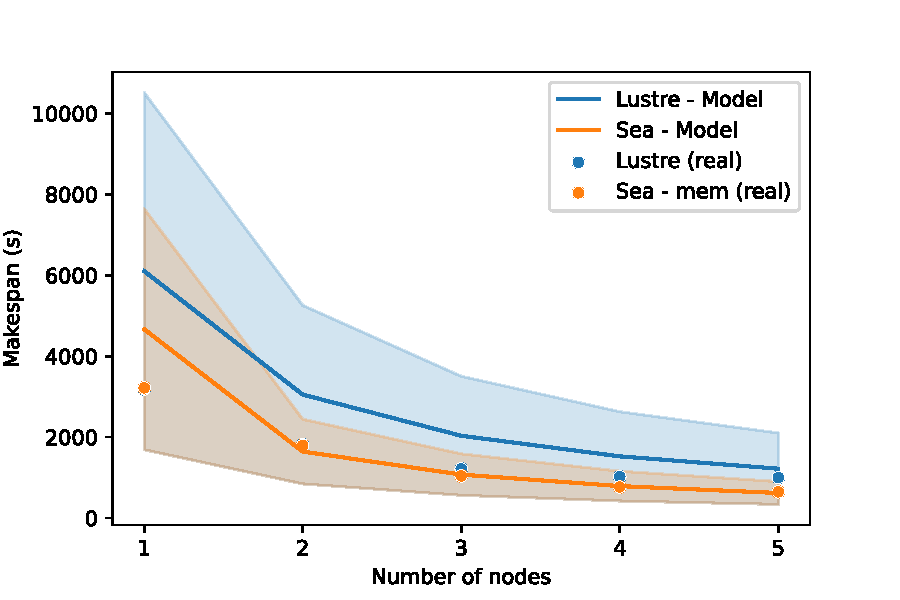
\includegraphics[width=0.8\linewidth]{figures/nodes.pdf}
            \caption{Experiment 1: Nodes}
            \label{fig:nodes}
        \end{subfigure}%
        \begin{subfigure}{0.5\textwidth}
            \centering
            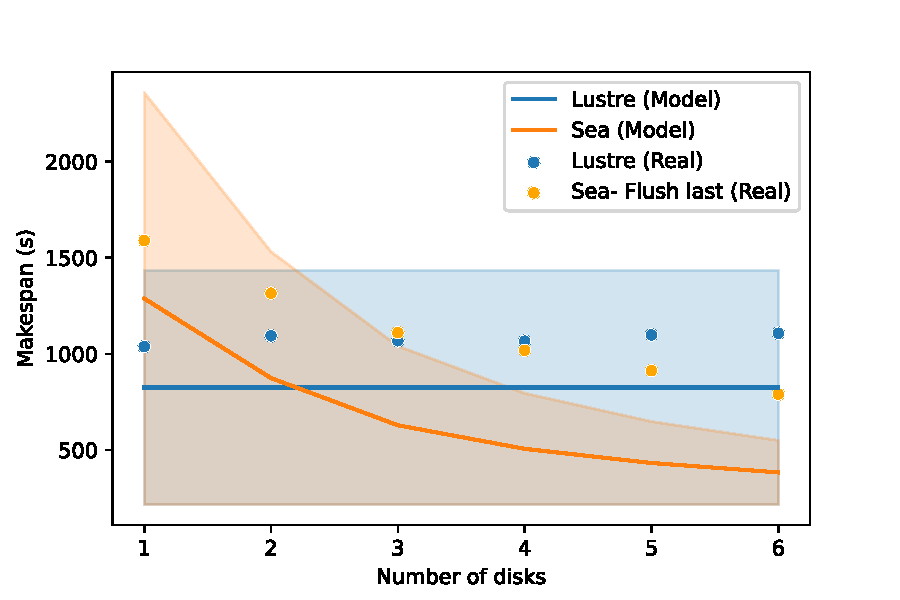
\includegraphics[width=0.8\linewidth]{figures/disks.pdf}
            \caption{Experiment 2: Disks}
            \label{fig:disks}
        \end{subfigure}
        \begin{subfigure}{0.5\textwidth}
            \centering
            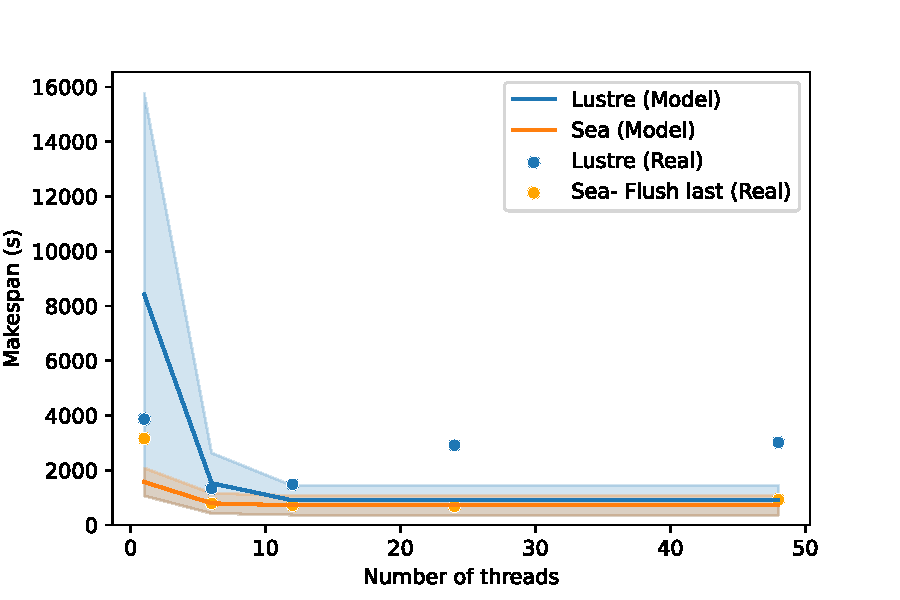
\includegraphics[width=0.8\linewidth]{figures/threads.pdf}
            \caption{Experiment 3: Threads}
            \label{fig:threads}
        \end{subfigure}
        \begin{subfigure}{0.5\textwidth}
            \centering
            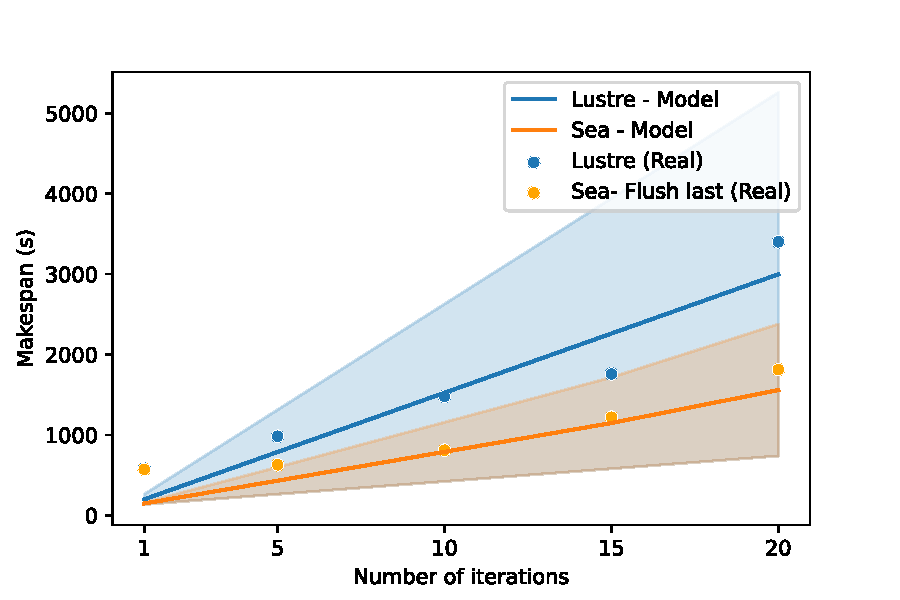
\includegraphics[width=0.8\linewidth]{figures/iterations.pdf}
            \caption{Experiment 4: Iterations}
            \label{fig:iterations}
        \end{subfigure}
        \caption{File system and model evaluation of Sea and Lustre. Shaded
        area represents makespan range, as determined by the model, with the
        lines representing the average of the bounds.}

    \label{fig:seaexp}
\end{figure}
    For the most part, the model appears to correctly encapsulate the
    performance range of Sea and Lustre, often times with the real data being
    situated at the halfway point between the min and max performance bounds.
    However, there are some notable exceptions.
    In Figure~\ref{fig:disks}, the model appears to adequately describe the
    performance of 1 and 2 disks, but the real results progressively surpass
    makespan estimates as the number of disks increases further. Model estimates
    for Lustre, however, encapsulate the results obtained. Interestingly
    enough, curve of the mid point line seems to parallel that of the results.

    Model estimates appear to be inaccurate to for Experiment 3, as seen in
    Figure~\ref{fig:threads}. For 1 and 6 threads, the results occur within
    the bounds of the model, however, at 12 threads, the real results start
    to exceed model estimates and then plateau at somewhere around 24 threads.

    In Figure~\ref{fig:iterations}, although model and results appear to
    generally be in accordance with each other, the model captures neither
    Sea's or Lustre's actual makespan. Furthermore, it is unclear from the
    results if the trend is actually linear.

    The greatest overall speedup occurred in Experiment 4 at 24 threads. In 
    this experiment, Sea was 4.3~x faster than the same conditions on Lustre.
    The second highest speedup also occurred in Experiment 4, when using 48
    threads. Sea was approximately 3.3~x faster than its Lustre counterpart.
    Otherwise, the maximum speedup obtained with Sea was 1.5~x in Experiment 1,
    1.4~x in Experiment 2 and 1.9~x in Experiment 3.

    In general, Sea's performance was not worse than that of Lustre's. The only
    time there was a noticeable decrease in performance occurred in Experiment 2
    when the number of disks used was below 3. This is a result of there being
    a greater contention on local storage with a reduced number of disks. While
    the local storage device bandwidths exceed that of Lustre \gls{ost}s (Table~\ref{table:fs}), Lustre has significantly more disks available that the overall
    attainable bandwidth is greater than that of local storage. Furthermore, 
    the network bandwidth to Lustre is also superior to the combined local
    storage bandwidth.

    \section{Discussion}\label{discussion}

    Overall, our results show that Sea performs better than Lustre when there is
    increased contention on Lustre as compared to the local storage devices. We
    expect that contention to Lustre will be significantly greater on a 
    production cluster where many users are accessing Lustre at the same time.
    As this may be the case, we might even expect Sea to outperform Lustre when
    processing data in a sequential application. However, as can be seen in
    Figure~\ref{fig:disks}, when local storage contention is greater than that
    of Lustre's, it is not recommended to use Sea. To circumvent this issue
    such that a user would not need prior knowledge on file system usage trends
    before deciding whether or not to use Sea, Sea could periodically benchmark
    the different file systems to ensure that the file is written to the most
    appropriate location.






    \chapter{Conclusions and Future work}

\end{document}
